%%%%%%%%%%%%%%%%%%%%%%%%%%%%%%%%%%%%%%%%%%%%%%%%%%%%%%%%%%%%%%%%%%%%%%%%%%%%%%%%
%% Plantilla de memoria en LaTeX para la ETSIT - Universidad Rey Juan Carlos
%%
%% Por Gregorio Robles <grex arroba gsyc.urjc.es>
%%     Grupo de Sistemas y Comunicaciones
%%     Escuela Técnica Superior de Ingenieros de Telecomunicación
%%     Universidad Rey Juan Carlos
%% (muchas ideas tomadas de Internet, colegas del GSyC, antiguos alumnos...
%%  etc. Muchas gracias a todos)
%%
%% La última versión de esta plantilla está siempre disponible en:
%%     https://github.com/gregoriorobles/plantilla-memoria
%%
%% Para obtener PDF, ejecuta en la shell:
%%   make
%% (las imágenes deben ir en PNG o JPG)

%%%%%%%%%%%%%%%%%%%%%%%%%%%%%%%%%%%%%%%%%%%%%%%%%%%%%%%%%%%%%%%%%%%%%%%%%%%%%%%%

\documentclass[a4paper, 12pt]{book}
%\usepackage[T1]{fontenc}

\usepackage[a4paper, left=2.5cm, right=2.5cm, top=3cm, bottom=3cm]{geometry}
\usepackage{times}
\usepackage[utf8]{inputenc}
%\usepackage[latin1]{inputenc}
%\usepackage[spanish]{babel} % Comenta esta l�nea si tu memoria es en ingl�s
\usepackage{url}
%\usepackage[dvipdfm]{graphicx}
\usepackage{graphicx}
\usepackage{float}  %% H para posicionar figuras
\usepackage[breaklinks=true]{hyperref} %% Para marcadores
\usepackage[nottoc, notlot, notlof, notindex]{tocbibind} %% Opciones de �ndice
\usepackage{latexsym}  %% Logo LaTeX
\usepackage{csquotes}  %% Paquete para citas (displayquote)
\usepackage{amsthm}  %% Paquete para Teoremas
\usepackage{color}  %% Paquete para texto en color
\usepackage[normalem]{ulem}  %% Para tablas
\useunder{\uline}{\ul}{}  %% Para tablas
\usepackage{listings}  %% para código y comandos
\usepackage{pdfpages}  %% para incluir archivos PDF
\usepackage{enumerate}  %% Para enumerar
\usepackage[parfill]{parskip}  %% Párrafos
\definecolor{codegreen}{rgb}{0,0.6,0}
\definecolor{codegray}{rgb}{0.5,0.5,0.5}
\definecolor{codepurple}{rgb}{0.58,0,0.82}
\definecolor{backcolour}{rgb}{0.82,0.82,0.82}

\lstdefinestyle{mystyle}{
    backgroundcolor=\color{backcolour},
    commentstyle=\color{codegreen},
    keywordstyle=\color{magenta},
    numberstyle=\tiny\color{codegray},
    stringstyle=\color{codepurple},
    basicstyle=\ttfamily\footnotesize,
    breakatwhitespace=false,
    breaklines=true,
    captionpos=b,
    keepspaces=true,
    numbers=left,
    numbersep=5pt,
    showspaces=false,
    showstringspaces=false,
    showtabs=false,
    tabsize=2
}

\lstdefinestyle{mystylesmall}{
    backgroundcolor=\color{backcolour},
    commentstyle=\color{codegreen},
    keywordstyle=\color{magenta},
    numberstyle=\tiny\color{codegray},
    stringstyle=\color{codepurple},
    basicstyle=\ttfamily\scriptsize,
    breakatwhitespace=false,
    breaklines=true,
    captionpos=b,
    keepspaces=true,
    numbers=left,
    numbersep=5pt,
    showspaces=false,
    showstringspaces=false,
    showtabs=false,
    tabsize=2
}

\lstset{style=mystyle}

\title{Memoria del Proyecto}
\author{Miguel Ángel Fernández Sánchez}

\renewcommand{\baselinestretch}{1.5}  %% Interlineado

\begin{document}

%\renewcommand{\refname}{Bibliografía}  %% Renombrando
%\renewcommand{\appendixname}{Apéndice}

%%%%%%%%%%%%%%%%%%%%%%%%%%%%%%%%%%%%%%%%%%%%%%%%%%%%%%%%%%%%%%%%%%%%%%%%%%%%%%%%
% PORTADA

\begin{titlepage}
\begin{center}
\begin{tabular}[c]{c c}
%\includegraphics[bb=0 0 194 352, scale=0.25]{logo} &
\includegraphics[scale=0.25]{img/logo_vect.png} &
\begin{tabular}[b]{l}
\Huge
\textsf{UNIVERSIDAD} \\
\Huge
\textsf{REY JUAN CARLOS} \\
\end{tabular}
\\
\end{tabular}

\vspace{3cm}

\Large
MÁSTER EN DATA SCIENCE

\vspace{0.4cm}

\large
Curso Académico 2020/2021

\vspace{0.8cm}

Trabajo Fin de Máster

\vspace{1.5cm}

\LARGE

IDENTIFICACIÓN AUTOMÁTICA DE CUENTAS BOT EN PROYECTOS \textit{OPEN-SOURCE}

% http://dl.acm.org/citation.cfm?id=2976778
\vspace{3cm}

\large
Autor : Miguel Ángel Fernández Sánchez \\
Tutor : Dr. Felipe Ortega
\end{center}
\end{titlepage}

\newpage
\mbox{}
\thispagestyle{empty} % para que no se numere esta pagina


%%%%%%%%%%%%%%%%%%%%%%%%%%%%%%%%%%%%%%%%%%%%%%%%%%%%%%%%%%%%%%%%%%%%%%%%%%%%%%%%
%%%% Para firmar
\clearpage
\pagenumbering{gobble}
%\chapter*{Evaluation}

\vspace{-4cm}
\begin{center}
\LARGE
\textbf{Trabajo Fin de Máster}

\vspace{1cm}
\large

TÍTULO

\vspace{1cm}
\large
\textbf{Autor :} Miguel Ángel Fernández Sánchez \\
\textbf{Tutor :} Dr. Felipe Ortega Soto 

\end{center}

\vspace{1cm}
La defensa del presente Trabajo Fin de Máster se realizó el día \qquad$\;\,$ de \qquad\qquad\qquad\qquad \newline de 2021, siendo calificada por el siguiente tribunal:


\vspace{0.5cm}
\textbf{Presidente:}

\vspace{1.2cm}
\textbf{Secretario:}

\vspace{1.2cm}
\textbf{Vocal:}


\vspace{1.2cm}
y habiendo obtenido la siguiente calificación:

\vspace{1cm}
\textbf{Calificación:}


\vspace{1cm}
\begin{flushright}
Madrid, a \qquad$\;\,$ de \qquad\qquad\qquad\qquad de 2021
\end{flushright}

%%%%%%%%%%%%%%%%%%%%%%%%%%%%%%%%%%%%%%%%%%%%%%%%%%%%%%%%%%%%%%%%%%%%%%%%%%%%%%%%
%%%% Dedicatoria

\chapter*{Dedications}
\pagenumbering{Roman} % para comenzar la numeracion de paginas en numeros romanos
\begin{flushright}

Dedicatoria

\end{flushright}
%%%%%%%%%%%%%%%%%%%%%%%%%%%%%%%%%%%%%%%%%%%%%%%%%%%%%%%%%%%%%%%%%%%%%%%%%%%%%%%%
%%%% Agradecimientos

\chapter*{Acknowledgements}
%\addcontentsline{toc}{chapter}{Agradecimientos} % si queremos que aparezca en el �ndice
\markboth{ACKNOWLEDGEMENTS}{ACKNOWLEDGEMENTS} % encabezado

Agradecimientos

%%%%%%%%%%%%%%%%%%%%%%%%%%%%%%%%%%%%%%%%%%%%%%%%%%%%%%%%%%%%%%%%%%%%%%%%%%%%%%%%
%%%% Resumen en ingl�s
\chapter*{Summary}
%\addcontentsline{toc}{chapter}{Summary} % si queremos que aparezca en el �ndice
\markboth{SUMMARY}{SUMMARY} % encabezado

Summary

%%%%%%%%%%%%%%%%%%%%%%%%%%%%%%%%%%%%%%%%%%%%%%%%%%%%%%%%%%%%%%%%%%%%%%%%%%%%%%%%
%%%% Resumen
\chapter*{Resumen}
%\addcontentsline{toc}{chapter}{Resumen} % si queremos que aparezca en el �ndice
\markboth{RESUMEN}{RESUMEN} % encabezado

Resumen

%%%%%%%%%%%%%%%%%%%%%%%%%%%%%%%%%%%%%%%%%%%%%%%%%%%%%%%%%%%%%%%%%%%%%%%%%%%%%%%%
%%%%%%%%%%%%%%%%%%%%%%%%%%%%%%%%%%%%%%%%%%%%%%%%%%%%%%%%%%%%%%%%%%%%%%%%%%%%%%%%
% �NDICES %
%%%%%%%%%%%%%%%%%%%%%%%%%%%%%%%%%%%%%%%%%%%%%%%%%%%%%%%%%%%%%%%%%%%%%%%%%%%%%%%%

% Las buenas noticias es que los �ndices se generan autom�ticamente.
% Lo �nico que tienes que hacer es elegir cu�les quieren que se generen,
% y comentar/descomentar esa instrucci�n de LaTeX.

%%%% �ndice de contenidos
\tableofcontents
%%%% �ndice de figuras
\cleardoublepage
%\addcontentsline{toc}{chapter}{Lista de figuras} % para que aparezca en el indice de contenidos
\listoffigures % indice de figuras
%%%% �ndice de tablas
%\cleardoublepage
%\addcontentsline{toc}{chapter}{Lista de tablas} % para que aparezca en el indice de contenidos
%\listoftables % indice de tablas

%%%%%%%%%%%%%%%%%%%%%%%%%%%%%%%%%%%%%%%%%%%%%%%%%%%%%%%%%%%%%%%%%%%%%%%%%%%%%%%%
%%%%%%%%%%%%%%%%%%%%%%%%%%%%%%%%%%%%%%%%%%%%%%%%%%%%%%%%%%%%%%%%%%%%%%%%%%%%%%%%
% INTRODUCCI�N %
%%%%%%%%%%%%%%%%%%%%%%%%%%%%%%%%%%%%%%%%%%%%%%%%%%%%%%%%%%%%%%%%%%%%%%%%%%%%%%%%

\cleardoublepage
\chapter{Introduction}
\label{sec:intro} % etiqueta para poder referenciar luego en el texto con ~\ref{sec:intro}
\pagenumbering{arabic} % para empezar la numeraci�n de p�gina con n�meros
% En este cap�tulo se introduce el proyeto. Deber�a tener informaci�n general sobre
% el mismo, dando la informaci�n sobre el contexto en el �que se ha desarrollado.
% No te olvides de echarle un ojo a la p�gina con los cinco errores de escritura m�s frecuentes\footnote{\url{http://www.tallerdeescritores.com/errores-de-escritura-frecuentes}}.

People contributing to software projects (in particular, FLOSS projects) rely on several tools to support their activity on many aspects of the project, such as source code changes, project management and coordination, software bugs and issues, etc.

The data generated by such interactions can be used to extract valuable information which can be used by project managers and leaders to take the right decisions for the future of the project (known as data-driven decisions). Some of the most common questions while analyzing an open-source project are:

\begin{itemize}
    \item How many contributors do we have? (Activity, Engagement)
    \item How many companies are contributing to my project? (Community, Diversity)
    \item How good we are in handling issues? (Processes, Efficiency) 
\end{itemize}

This data is also interesting for academic purposes, as researchers and practitioners may be interested in answering a set of questions about a given project.

\section{GrimoireLab}

GrimoireLab\footnote{\url{https://chaoss.github.io/grimoirelab/}} is a free, open source tool-set for software development analytics.
This tool-set provides a whole platform which supports automatic and incremental data gathering from many tools (data sources) related with Open Source development (source code management, issue tracking systems, messaging tools, mailing lists, etc.).
The data obtained from these tools is stored in JSON documents following a uniform format, no matter the source. These JSON documents are stored in Elasticsearch and go through a data enrichment process, adding additional information such time calculations (delays, duration), geographical data, contributors affiliation and more.
Once the data has been augmented, it can be consumed by visualization tools and also directly using the Elasticsearch API. GrimoireLab tool-set comes with a tool named “Kibiter” which is a soft-fork of Elastic’s Kibana. A set of pre-defined dashboards and visualizations are included for each data source.  
GrimoireLab is part of CHAOSS, a project by The Linux Foundation. It is mainly developed by the Spanish company Bitergia, and it is an evolution of the work done during more than 10 years by Bitergia and the LibreSoft research group from Rey Juan Carlos University.

\section{SortingHat}

From a project management perspective, a person (generally with a manager role) needs to know their community or project. In order  to get valuable insights, that person may end up asking two main questions:

\begin{itemize}
    \item How many contributors does the project has?
    \item How many organizations are contributing to the project?
\end{itemize}

To answer these questions, we need to manage contributor identities within the project.

After spotting the usage of a plethora of different tools within FLOSS projects, it is important to explain that, for interacting with each of these tools, each contributor to the project is required to be identified in some way. This could be done by creating an account or setting up a set of credentials, which usually are a combination of name and email. This means each contributor will end up with one or more different “accounts” or “identities” for the services the project is using.

In such a scenario, it could happen that some contributors are using more than one account or set of credentials (from now on, we will refer to these as identities) for the same tool or service, for instance to differentiate the contributions made from an organizational account and those made from a personal or academic account. We name as individual as the entity representing the many identities of a contributor, its profile and enrollment information. This problem alone entails one of the hardest problems to solve: proper identity merging.

Furthermore, some of these identities can belong to automatic processes which fulfil a predefined set of tasks within the tool or service. For instance, (examples). 

SortingHat is the GrimoireLab component which aims to help and simplify the identity management within a project or set of projects. It provides more than 20 commands to manipulate identities, including support for (i) identity merging based on email addresses, usernames and full names found on many tools used in software development, (ii) enrolling members to organizations for a given time span, marking identities as automatic accounts (Bots) and (iii) gender assessment, among other features.

This tool maintains a relational database with identities and related information extracted from different tools used in software development [3]. An identity is a tuple composed of a name, email, username and the name of the source from where it was extracted. Tuples are converted to unique identifiers (i.e., uuid), which provide a quick mean to compare identities among each other. By default, SortingHat considers all identities as unique ones. Heuristics take care to automatically merge identities based on perfect matches on \((i)\) uuids, \((ii)\) name, \((iii)\) email or \((iv)\) username.

In case of a positive match, an identity is randomly selected as the unique one, and the other identities are linked to it.

\begin{figure}
 \centering
  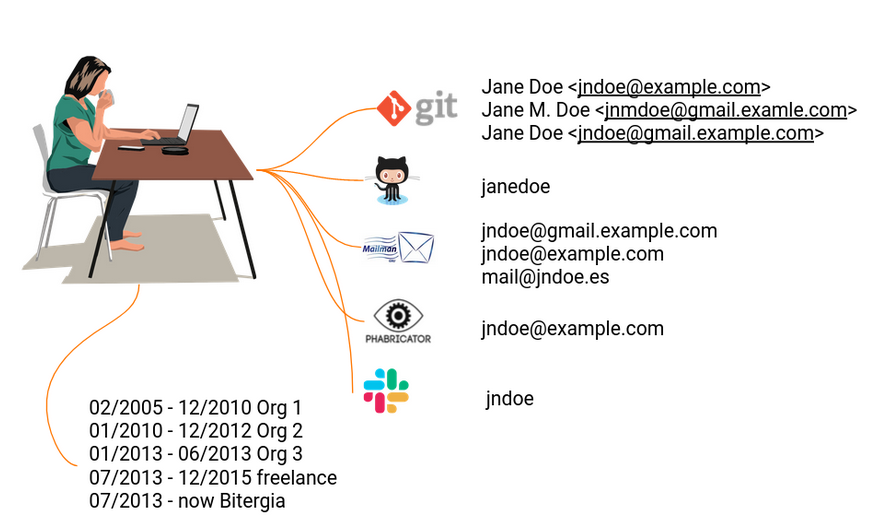
\includegraphics[width=12cm, keepaspectratio]{img/example-identity}
  \caption{A project contributor can have many identities and affiliation information}
  \label{fig:example-identity}
\end{figure}

\section{Automatic accounts: Bots}

It is important to state that some of the interactions which occur within the tools used for software development are not created directly by humans: they are a result of an automated process set with a specific purpose and level of permission to produce a specific output affecting the state of the project and its members.

Although this type of interactions does not appear in all open source projects, they are very common (reference?) within the projects from top-level communities such GitLab (link, reference), Wikimedia Foundation (link, reference), OpenStack (link, reference) and more.

The number of Bot accounts and the amount of their interactions depend on many factors:
\begin{itemize}
    \item Type and purpose of the tool or service (issue management, messaging, bug tracker, etc.)
    \item If this is an option provided by default by the tool or it is a feature developed ad-hoc.
    \item How this automatic accounts (Bots) are configured: Triggered by events, periodic execution, etc.
    \item The amount of activity generated by humans or by other automatic accounts within the project.
    \item ...
\end{itemize}

Although SortingHat provides a way to mark unique idenities as “Bot” accounts by editing the identity’s profile (setting up a boolean field named \texttt{is\_bot}), there is not an automated way to identify which individuals from the whole data set could be marked as “Bots”.

Up to now, this is an entire manual process and requires time from a person actively searching for suspicious identities of being “Bot” accounts, looking at some key values such as their username, email or type of contributions, together with more research by checking the original source of the data, looking for extra information which can help to verify the operator’s guesses.

On this thesis, it is proposed an approach to identify individuals from Automatic accounts (Bots) using machine learning techniques to build a classifier based on the contributions produced by all the identities from a given set of projects. This classifier will be integrated as an additional SortingHat feature integrated with the own recommendation engine the tool already has implemented.

%%%%%%%%%%%%%%%%%%%%%%%%%%%%%%%%%%%%%%%%%%%%%%%%%%%%%%%%%%%%%%%%%%
\section{Structure of the thesis}
\label{sec:structure}



%%%%%%%%%%%%%%%%%%%%%%%%%%%%%%%%%%%%%%%%%%%%%%%%%%%%%%%%%%%%%%%%%%%%%%%%%%%%%%%%
%%%%%%%%%%%%%%%%%%%%%%%%%%%%%%%%%%%%%%%%%%%%%%%%%%%%%%%%%%%%%%%%%%%%%%%%%%%%%%%%
% OBJETIVOS %
%%%%%%%%%%%%%%%%%%%%%%%%%%%%%%%%%%%%%%%%%%%%%%%%%%%%%%%%%%%%%%%%%%%%%%%%%%%%%%%%
\cleardoublepage
\chapter{Objectives}
\label{sec:objectives}

The main objective of this project is to find out if there is a way to set up an automatic or semi-automatic way to classify individuals from GrimoireLab’s SortingHat into human users and Bot accounts.

This should be done by obtaining data from each individual, from specific channels (data sources) where it will be studied which variables are relevant to make this classification effective.

\section{GQM approach}

The "Goal Question Metric" (GQM) approach\footnote{“The Goal Question Metric Approach”, Basili, Victor R. and Caldiera, Gianluigi and Rombach, Dieter H., Encyclopedia of Software Engineering, John Wiley & Sons, 1994. \url{http://www.cs.umd.edu/~mvz/handouts/gqm.pdf}} is based upon the assumption that for an organization to measure in a purposeful way it must first specify the goals for itself and its projects, then it must trace those goals to the data that are intended to define those goals operationally, and finally provide a framework for interpreting the data with respect to the stated goals.

This approach helps to define the metrics that matter in each case, avoiding some usual bad practices. For instance, people tend to use or define a set of metrics without having a clear idea about the specific goals they pursue. This usually leads to have a "bottom-up" approach: besides having metrics misaligned with project or business goals, the set of metrics may be biased by the current technology used to obtain these metrics.

Not having a defined strategy also hinders people to understand which metrics are important and why. By using a "top-down" approach (first goals, then metrics), it is easier to materialize the appropriate set of questions for the current situation, and then check which metrics could be useful in the future or not and how these metrics helped to reach the different goals by answering the questions that were raised.

\begin{figure}
 \centering
  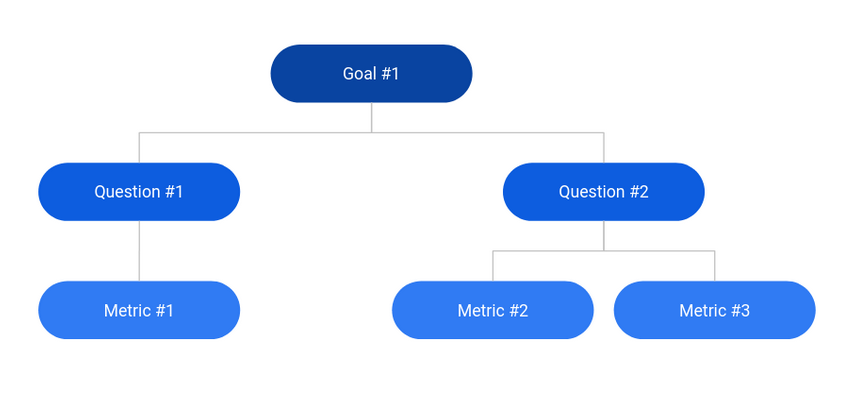
\includegraphics[width=12cm, keepaspectratio]{img/example-gqm-schema}
  \caption{Example: Goal, Question, Metric approach hierarchy}
  \label{fig:example-gqm-schema}
\end{figure}

\section{Goals and Questions}

\textbf{Goal 1}: Have an automatic process to discriminate between human users and Bot accounts, integrated into the GrimoireLab toolset.

\begin{itemize}
    \item \textbf{Q1.1.} How to separate bot accounts from human users?
    \item \textbf{Q1.2.} Is the profile information from a given individual enough to classify it as human or Bot?
    \item \textbf{Q1.3.} Are there differences between the activity generated by humans and bots?
    \item \textbf{Q1.4.} How can this classifier be integrated within GrimoireLab’s tool chain?
\end{itemize}

\textbf{Goal 2}: Find which channels and footprints can be used to classify an user as human or Bot.

\begin{itemize}
    \item \textbf{Q2.1.} Are there any particular channels and footprints (huella digital), as a combination of interactions which can be used to classify a user as human or bot?
    \item \textbf{Q2.2.} Message content (commit messages, issue texts, etc.) can be used to validate this classification?
    \begin{itemize}
        \item \textbf{Q2.2.1.} Does a richer syntax give a hint about the nature of the user? 
        \item \textbf{Q2.2.2.} Can the entropy of a comment give a hint about the nature of the user? \begin{itemize}
            \item \textbf{Hypothesis}: Humans have more entropy when they write comments. Problem: use of templates. Note: Use Spacy.
        \end{itemize}
    \end{itemize}
    \item \textbf{Q2.3.} Do working hours and frequency of contributions help on this classification?

\end{itemize}

\textbf{Goal 3}: Get a curated dataset from real OpenSource communities with real examples of Bot accounts.

\begin{itemize}
    \item \textbf{Q3.1.} Which Open-source communities should be analyzed?
    \item \textbf{Q3.2.} Which data sources are we taking into account?
    \begin{itemize}
        \item \textbf{Q3.2.1.} From these data sources, which data should we consider?
    \end{itemize}
\end{itemize}

\textbf{Goal 4}: Extend the classifier to other OpenSource communities and other projects using Bot accounts.

\begin{itemize}
    \item \textbf{Q4.1.} Once the classifier is trained for a given Open-source project, is the result valid for other projects from the same community?
    \item \textbf{Q4.2.} Once the classifier is trained for a given Open-source project, is the result valid for other projects from other communities?
\end{itemize}

\textbf{Goal 5}: Classify Bot accounts into sub-categories, according to their role in the project.

\begin{itemize}
    \item \textbf{Q5.1.}: Inside the bot users, can we identify sub-categories? For instance, bots executing tests or reviewing critical parts of the system.
\end{itemize}

\section{Metrics}
For now, this is an initial list of metrics by channel.

\subsection{Git (commits), per individual}

\begin{itemize}
    \item \textbf{M1}: Number of modified files (mean, median)
    \item \textbf{M2}: Number of added lines (mean, median)
    \item \textbf{M3}: Number of removed lines (mean, median)
    \item \textbf{M4}: Does the commit have a message after the title? (boolean)
    \item \textbf{M5}: Length of the message? (mean, median)
    \item \textbf{M26}: Richness of the syntax
    \item \textbf{M6}: Is the commit verified? (git commit -s) (percentage? boolean?)
    \item \textbf{M29}: Extensions of modified files (areas of code) (number of distinct extensions?)
    \item \textbf{M7}: Commit frequency for each user (UTC date of the commit, define base period of time to consider)
    \item \textbf{M8}: Is the user active during the working days of the week? 
    \item \textbf{M9}: Is the user active during the weekend?
    \item \textbf{M10}: Does the user have a regular schedule? (e.g., there is a time from when the user is not active until the next day).
    \item \textbf{M11}: Name, email from the commit: Does any contain a keyword as bot?
\end{itemize}

Fields: \texttt{files}, \texttt{lines\_added}, \texttt{lines\_removed}, \texttt{utc\_commit}, \texttt{message}, \texttt{committer\_name}.

\subsection{GitHub Issues, per individual}

\begin{itemize}
    \item \textbf{M12}: Number of issues created by each user (define period of time)
    \item \textbf{M13}: Number of comments (mean, median) for each user, issue or period of time
    \item \textbf{M14}: Number of reactions (mean, median) for each user, issue or period of time
    \item \textbf{M28}: Number of distinct reactions.
    \item \textbf{M15}: Frecuency of issue creation (define base period of time)
    \item \textbf{M16}: Does the user create PRs too?
    \item \textbf{M17}: Does the user create PRs on the same repository where that user submitted commits?
    \item \textbf{M18}: Does the user create issues on the same repository where that user submitted commits?
    \item \textbf{M8}: Is the user active during the working days of the week? 
    \item \textbf{M9}: Is the user active during the weekend?
    \item \textbf{M10}: Does the user have a regular schedule? (e.g., there is a time from when the user is not active until the next day).
    \item \textbf{M11}: User name, does any contain a keyword as bot? 
    \item \textbf{M26}: Richness of the syntax (comments)
    \item \textbf{M27}: Entropy of the text (comments)
\end{itemize}

Fields: \texttt{grimoire\_creation\_date}, \texttt{pull\_request}, \texttt{title}, \texttt{user\_name}, \texttt{user\_login}, \texttt{url}, \texttt{repository}, \texttt{state}, \texttt{time\_open\_days}, \texttt{time\_to\_close\_days}, \texttt{time\_to\_first\_attention}, \texttt{tag}.

\subsection{GitHub Pull Requests, per individual}

\begin{itemize}
    \item \textbf{M19}: Number of PRs created by each user (define period of time)
    \item \textbf{M20}: Number of PRs merged by each user (define period of time)
    \item \textbf{M13}: Number of comments (mean, median) for each user, PR or period of time
    \item \textbf{M21}: From these comments, how many are review comments?
    \item \textbf{M14:} Number of reactions (mean, median) for each user, PR or period of time
    \item \textbf{M28}: Number of distinct reactions.
    \item \textbf{M22}: Frecuency of PRs creation (define base period of time)
    \item \textbf{M23}: Does the user create Issues too?
    \item \textbf{M24}: Does the user create Issues on the same repository where that user submitted commits?
    \item \textbf{M25}: Does the user create PRs on the same repository where that user submitted commits?
    \item \textbf{M8}: Is the user active during the working days of the week? 
    \item \textbf{M9}: Is the user active during the weekend?
    \item \textbf{M10}: Does the user have a regular schedule? (e.g., there is a time from when the user is not active until the next day).
    \item \textbf{M11}: User name, does any contain a keyword as bot? 
    \item \textbf{M26}: Richness of the syntax (comments)
    \item \textbf{M27}: Entropy of the text (comments)
\end{itemize}

Fields: \texttt{grimoire\_creation\_date}, \texttt{pull\_request}, \texttt{title}, \texttt{user\_name}, \texttt{user\_login}, \texttt{url}, \texttt{repository}, \texttt{state}, \texttt{time\_open\_days}, \texttt{time\_to\_close\_days}, \texttt{time\_to\_first\_attention}, \texttt{tag}.

\section{Technical proposal}

%%%%%%%%%%%%%%%%%%%%%%%%%%%%%%%%%%%%%%%%%%%%%%%%%%%%%%%%%%%%%%%%%%%%%%%%%%%%%%%%
%%%%%%%%%%%%%%%%%%%%%%%%%%%%%%%%%%%%%%%%%%%%%%%%%%%%%%%%%%%%%%%%%%%%%%%%%%%%%%%%
% ESTADO DEL ARTE %
%%%%%%%%%%%%%%%%%%%%%%%%%%%%%%%%%%%%%%%%%%%%%%%%%%%%%%%%%%%%%%%%%%%%%%%%%%%%%%%%
\cleardoublepage
\chapter{State of the art}
\label{sec:state-art}
%Puedes citar libros, como el de Bonabeau et al. sobre procesos estigm�rgicos~\cite{bonabeau:_swarm}.
 % Nota que el ~ a�ade un espacio en blanco, pero no deja que exista un salto de l�nea. Imprescindible ponerlo para las citas.
%%%%%%%%%%%%%%%%%%%%%%%%%%%%%%%%%%%


%%%%%%%%%%%%%%%%%%%%%%%%%%%%%%%%%%%%%%%%%%%%%%%%%%%%%%%%%%%%%%%%%%%%%%%%%%%%%%%%
%%%%%%%%%%%%%%%%%%%%%%%%%%%%%%%%%%%%%%%%%%%%%%%%%%%%%%%%%%%%%%%%%%%%%%%%%%%%%%%%
% DISEÑO E IMPLEMENTACIÓN %
%%%%%%%%%%%%%%%%%%%%%%%%%%%%%%%%%%%%%%%%%%%%%%%%%%%%%%%%%%%%%%%%%%%%%%%%%%%%%%%%
\cleardoublepage
\chapter{Design and implementation}
\label{sec:design-implementation}


%%%%%%%%%%%%%%%%%%%%%%%%%%%%%%%%%%%%%%%%%%%%%%%%%%%%%%%%%%%%%%%%%%%%%%%%%%%%%%%%
%%%%%%%%%%%%%%%%%%%%%%%%%%%%%%%%%%%%%%%%%%%%%%%%%%%%%%%%%%%%%%%%%%%%%%%%%%%%%%%%
% RESULTADOS %
%%%%%%%%%%%%%%%%%%%%%%%%%%%%%%%%%%%%%%%%%%%%%%%%%%%%%%%%%%%%%%%%%%%%%%%%%%%%%%%%
\cleardoublepage
\chapter{Results}
\label{sec:results}


%%%%%%%%%%%%%%%%%%%%%%%%%%%%%%%%%%%%%%%%%%%%%%%%%%%%%%%%%%%%%%%%%%%%%%%%%%%%%%%%
%%%%%%%%%%%%%%%%%%%%%%%%%%%%%%%%%%%%%%%%%%%%%%%%%%%%%%%%%%%%%%%%%%%%%%%%%%%%%%%%
% CONCLUSIONES %
%%%%%%%%%%%%%%%%%%%%%%%%%%%%%%%%%%%%%%%%%%%%%%%%%%%%%%%%%%%%%%%%%%%%%%%%%%%%%%%%
\cleardoublepage
\chapter{Conclusions}
\label{sec:conclusions}


%%%%%%%%%%%%%%%%%%%%%%%%%%%%%%%%%%%
\section{Achieved objectives}
\label{sec:achieved-objectives}

%%%%%%%%%%%%%%%%%%%%%%%%%%%%%%%%%%%
\section{Knowledge application}
\label{sec:knowledge-application}


%%%%%%%%%%%%%%%%%%%%%%%%%%%%%%%%%%%
\section{Learning outcomes}
\label{sec:learning-outcomes}
These are some of the learning outcomes I have reached thank to this project:


%%%%%%%%%%%%%%%%%%%%%%%%%%%%%%%%%%%
\section{Future work}
\label{sec:future-work}



%%%%%%%%%%%%%%%%%%%%%%%%%%%%%%%%%%%
\section{Personal assessment}
\label{sec:assessment}


%%%%%%%%%%%%%%%%%%%%%%%%%%%%%%%%%%%%%%%%%%%%%%%%%%%%%%%%%%%%%%%%%%%%%%%%%%%%%%%%
% BIBLIOGRAFIA %
%%%%%%%%%%%%%%%%%%%%%%%%%%%%%%%%%%%%%%%%%%%%%%%%%%%%%%%%%%%%%%%%%%%%%%%%%%%%%%%%
\cleardoublepage
% Las siguientes dos instrucciones es todo lo que necesitas
% para incluir las citas en la memoria
\bibliographystyle{abbrv}
\bibliography{memoria}  % memoria.bib es el nombre del fichero que contiene
% las referencias bibliogr�ficas. Abre ese fichero y mira el formato que tiene,
% que se conoce como BibTeX. Hay muchos sitios que exportan referencias en
% formato BibTeX. Prueba a buscar en http://scholar.google.com por referencias
% y ver�s que lo puedes hacer de manera sencilla.
% M�s informaci�n:
% http://texblog.org/2014/04/22/using-google-scholar-to-download-bibtex-citations/


%%%%%%%%%%%%%%%%%%%%%%%%%%%%%%%%%%%%%%%%%%%%%%%%%%%%%%%%%%%%%%%%%%%%%%%%%%%%%%%%
%%%%%%%%%%%%%%%%%%%%%%%%%%%%%%%%%%%%%%%%%%%%%%%%%%%%%%%%%%%%%%%%%%%%%%%%%%%%%%%%
% APPENDIX %
%%%%%%%%%%%%%%%%%%%%%%%%%%%%%%%%%%%%%%%%%%%%%%%%%%%%%%%%%%%%%%%%%%%%%%%%%%%%%%%%
\cleardoublepage
\appendix
%%%%%%%%%%%%%%%%%%%%%%%%%%%%%%%%%%%%%%%%%%%%%%%%%%%%%%%%%%%%%%%%%%%%%%%%%%%%%%%%
%%%%%%%%%%%%%%%%%%%%%%%%%%%%%%%%%%%%%%%%%%%%%%%%%%%%%%%%%%%%%%%%%%%%%%%%%%%%%%%%
% DEFINITIONS %
%%%%%%%%%%%%%%%%%%%%%%%%%%%%%%%%%%%%%%%%%%%%%%%%%%%%%%%%%%%%%%%%%%%%%%%%%%%%%%%%
\chapter{Definitions & Domain Knowledge}
\label{app:definitions}
%%%%%%%%%%%%%%%%%%%%%%%%%%%%%%%%%%%

%%%%%%%%%%%%%%%%%%%%%%%%%%%%%%%%%%%%%%%%%%%%%%%
\section{Essential freedoms of Free/Libre Software}
\label{sec:freedoms}
A program is free software if the program's users have the four essential freedoms:
\begin{itemize}
   \item The freedom to run the program as you wish, for any purpose (freedom 0).
   \item The freedom to study how the program works, and change it so it does your computing as you wish (freedom 1).
   \item The freedom to redistribute copies (freedom 2).
   \item The freedom to distribute copies of your modified versions to others (freedom 3).
\end{itemize}
A program is free software if it gives users adequately all of these freedoms. Otherwise, it is \textit{nonfree} or \textit{propietary}.
%%%%%%%%%%%%%%%%%%%%%%%%%%%%%%%%%%%
%%%%%%%%%%%%%%%%%%%%%%%%%%%%%%%%%%%%%%%%%%%%%%%%%%%%%%%%%%%%%%%%%%%%%%%%%%%%%%%%
% CODE %
%%%%%%%%%%%%%%%%%%%%%%%%%%%%%%%%%%%%%%%%%%%%%%%%%%%%%%%%%%%%%%%%%%%%%%%%%%%%%%%%
\chapter{Code of the tool}
\label{app:code}

%%%%%%%%%%%%%%%%%%%%%%%%%%%%%%%%%%%%%%%%%%%%%%%%%%%%%%%%%%%%%%%%%%%%%%%%%%%%%%%%
\end{document}
